% 12pt .6pt grayscale fragment
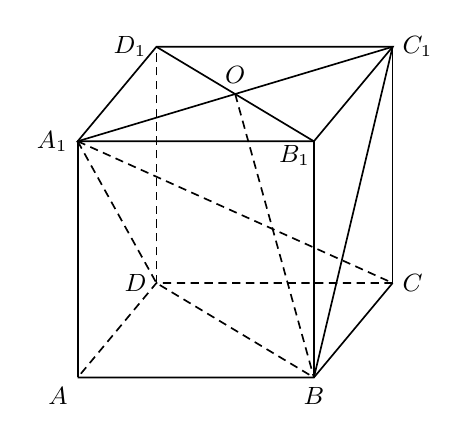
\begin{tikzpicture}[line width=.6pt, font=\small]
\coordinate (A) at (0,0);
\coordinate (B) at (3,0);
\coordinate (C) at (4,1.2);
\coordinate (D) at (1,1.2);
\coordinate (A1) at (0,3);
\coordinate (B1) at (3,3);
\coordinate (C1) at (4,4.2);
\coordinate (D1) at (1,4.2);
\coordinate (O) at (2,3.6);
\draw[densely dashed] (C)--(D)--(A);
\draw (A)--(A1);
\draw[densely dashed] (D)--(D1);
\draw (A)--(B)--(C);
\draw (B)--(B1);
\draw (C)--(C1);
\draw (A1)--(B1)--(C1)--(D1)--cycle;
\draw (A1)--(C1);
\draw (D1)--(B1);
\draw[densely dashed] (A1)--(D)--(B);
\draw (B)--(C1);
\draw[densely dashed] (A1)--(C);

\draw[densely dashed] (O)--(B);
\node[below left] at (A) {$A$};
\node[below] at (B) {$B$};
\node[right] at (C) {$C$};
\node[left] at (D) {$D$};
\node[left] at (A1) {$A_{1}$};
\node[below,xshift=-7pt,yshift=2pt] at (B1) {$B_{1}$};
\node[right] at (C1) {$C_{1}$};
\node[left] at (D1) {$D_{1}$};
\node[above] at (O) {$O$};
\end{tikzpicture}
